\section{Medições em laboratório}

No laboratório, montamos o circuito para realizar medições e analisar suas respostas a diversas frequências e amplitudes de sinal de entrada. Essa abordagem abrangente fornece informações práticas sobre o comportamento, estabilidade e desempenho do circuito em diferentes cenários operacionais, permitindo uma comparação posterior com as previsões teóricas.

\begin{figure}[H]
    \centering
    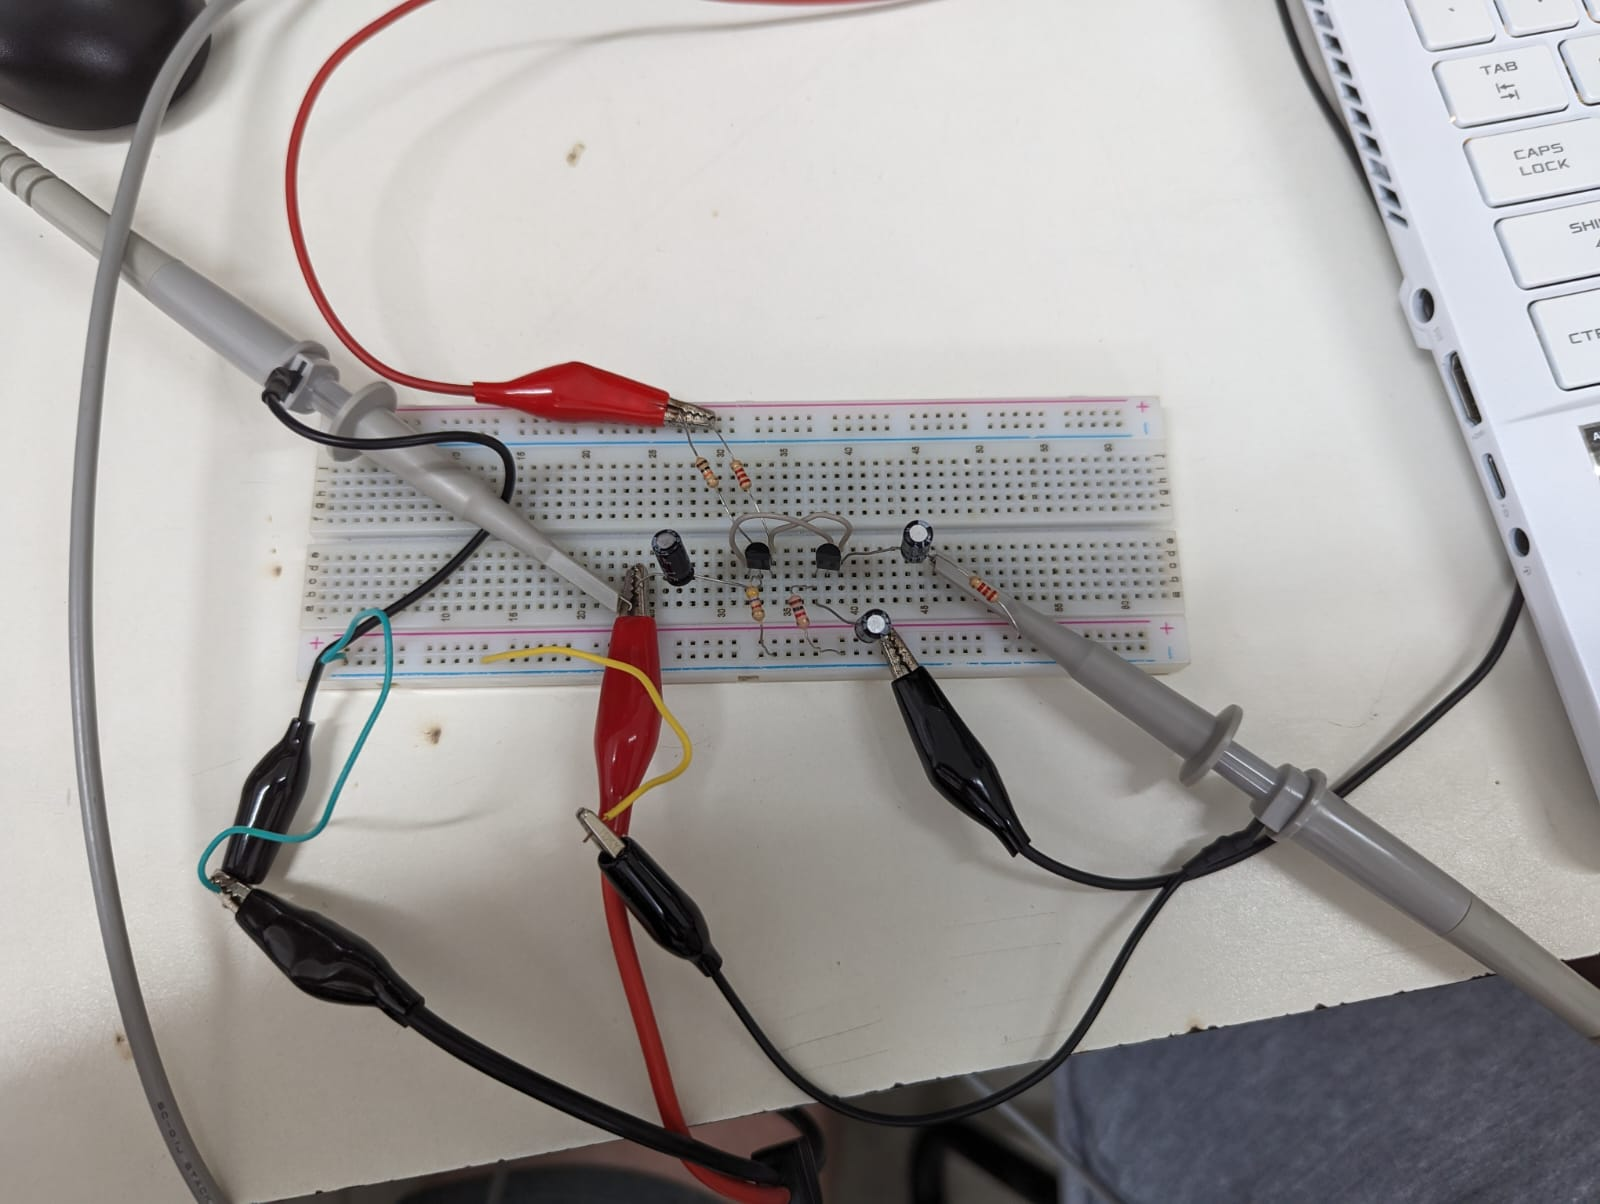
\includegraphics[width=0.5\columnwidth]{Images/circuito_real.jpeg}
    \caption{Circuito Darlington montado em laboratório.}
\end{figure}

\subsection{Tabela de componentes}

\begin{figure}[H]
    \centering
    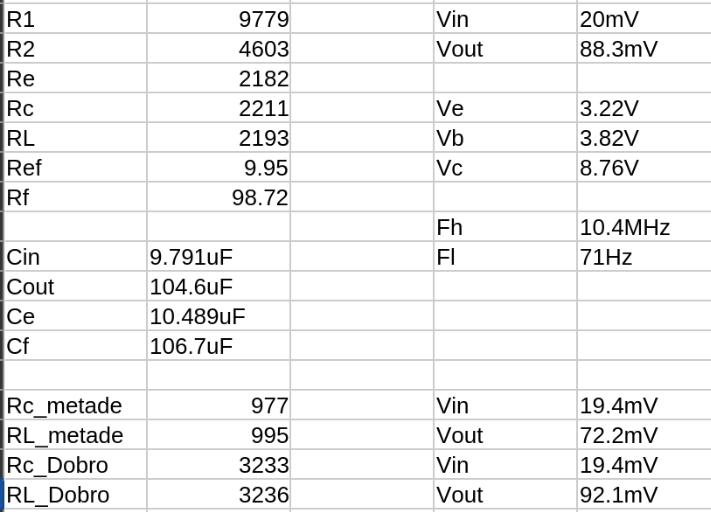
\includegraphics[width=0.5\columnwidth]{Images/componentes_reais.png}
    \caption{Valores dos componentes medidos em laboratório.}
\end{figure}

\subsection{Medidas sob diferentes condições}

\begin{figure}[H]
    \centering
    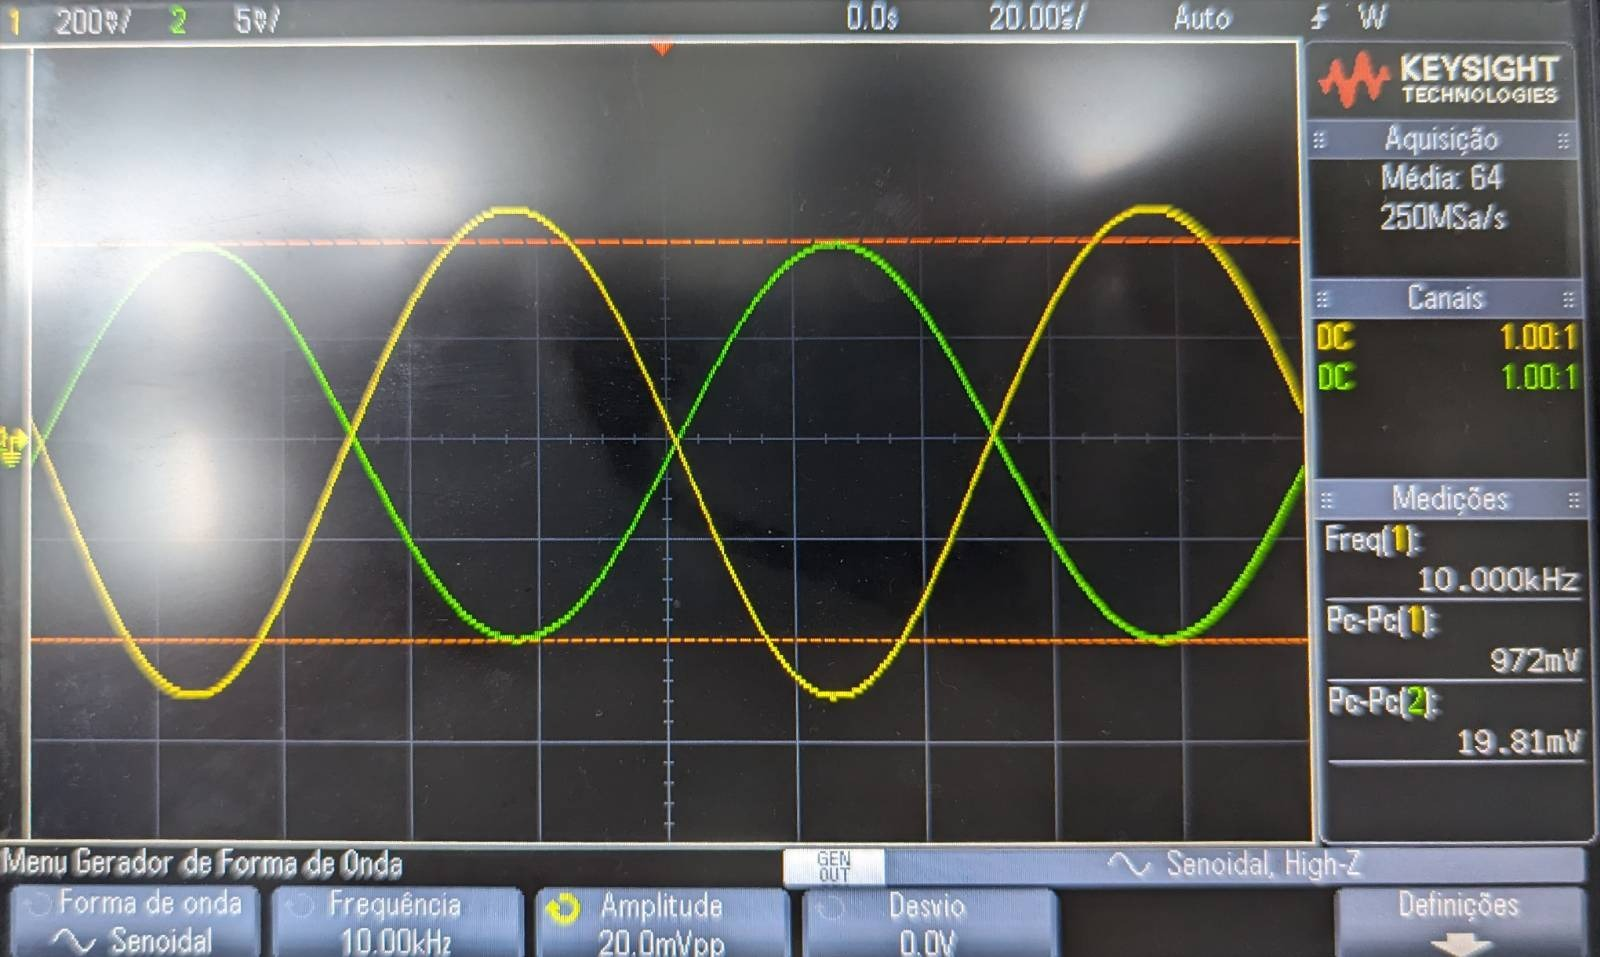
\includegraphics[width=0.5\columnwidth]{Images/ganho_do_circuito_normal.jpeg}
    \caption{Circuito com componentes e condições iniciais.}
\end{figure}

\begin{figure}[H]
    \centering
    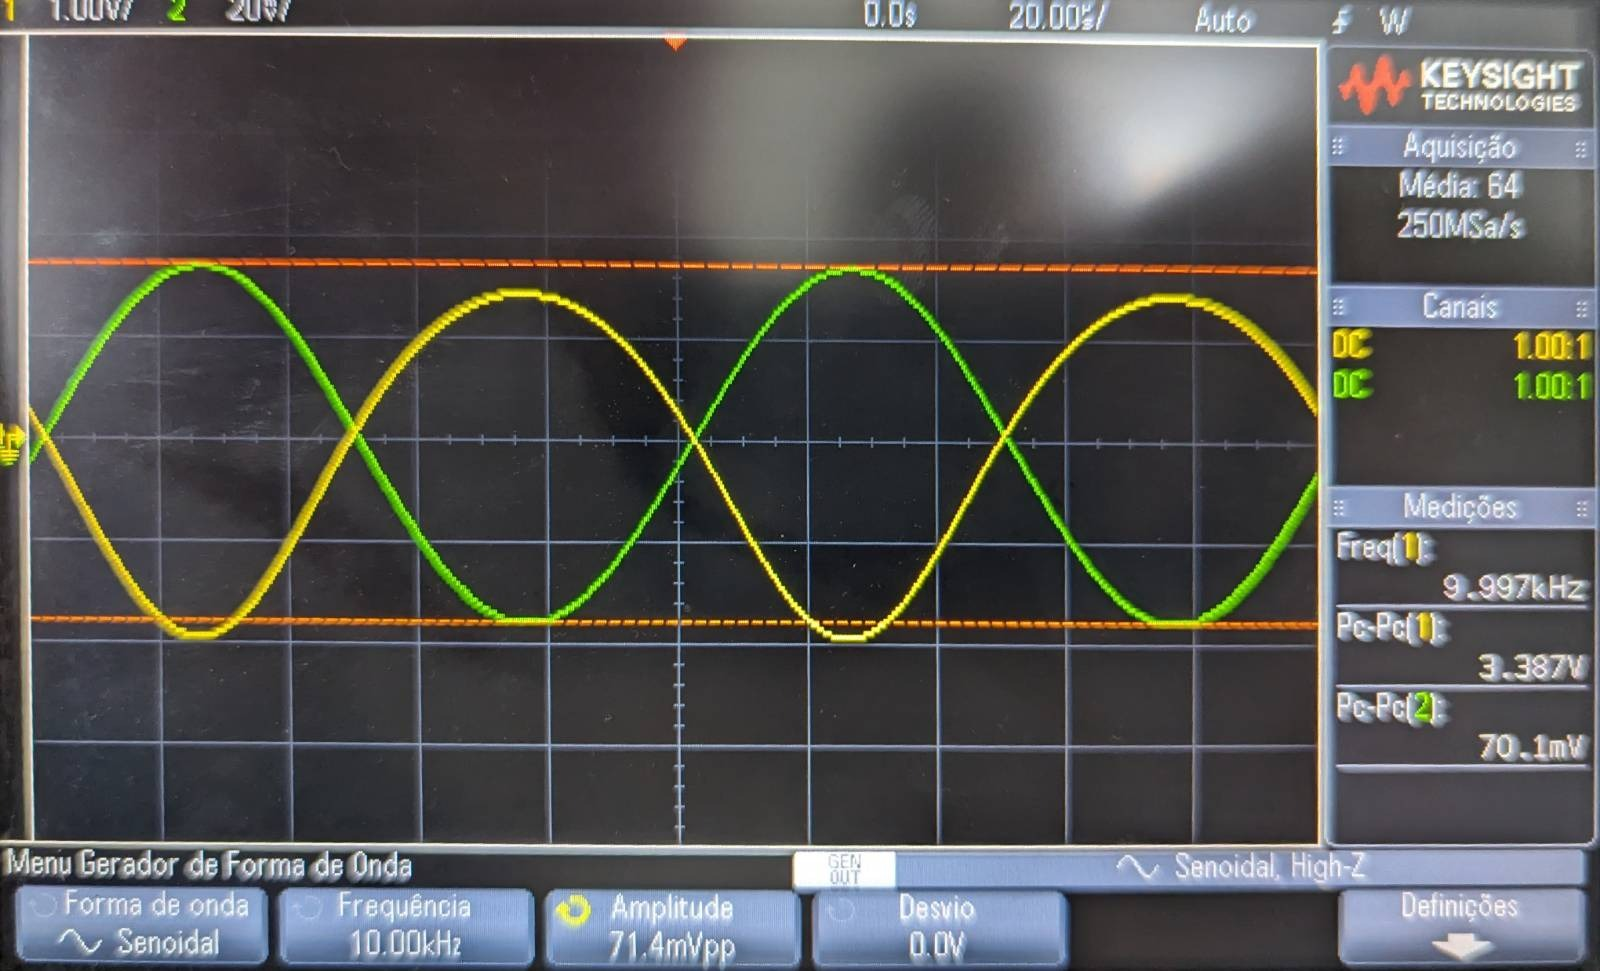
\includegraphics[width=0.5\columnwidth]{Images/circuito_inicio_saturacao.jpeg}
    \caption{Circuito em início de saturação após tensão ser aumentada.}
\end{figure}


\begin{figure}[H]
    \centering
    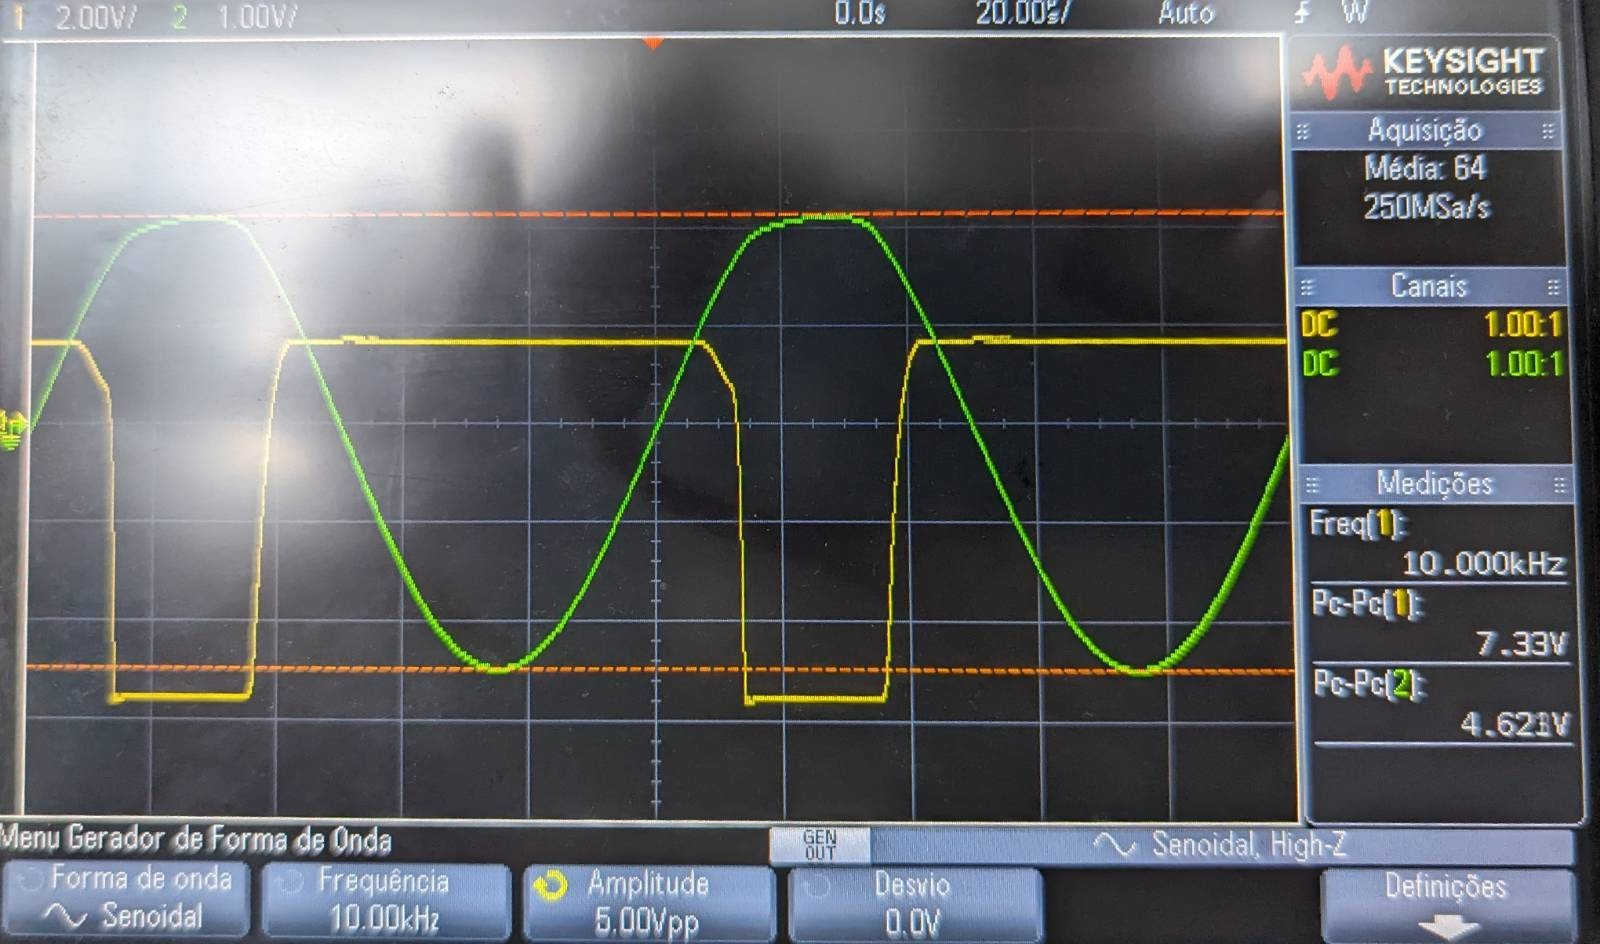
\includegraphics[width=0.5\columnwidth]{Images/saturacao_amplitude.jpeg}
    \caption{Circuito em saturação após tensão ser aumentada.}
\end{figure}

\begin{figure}[H]
    \centering
    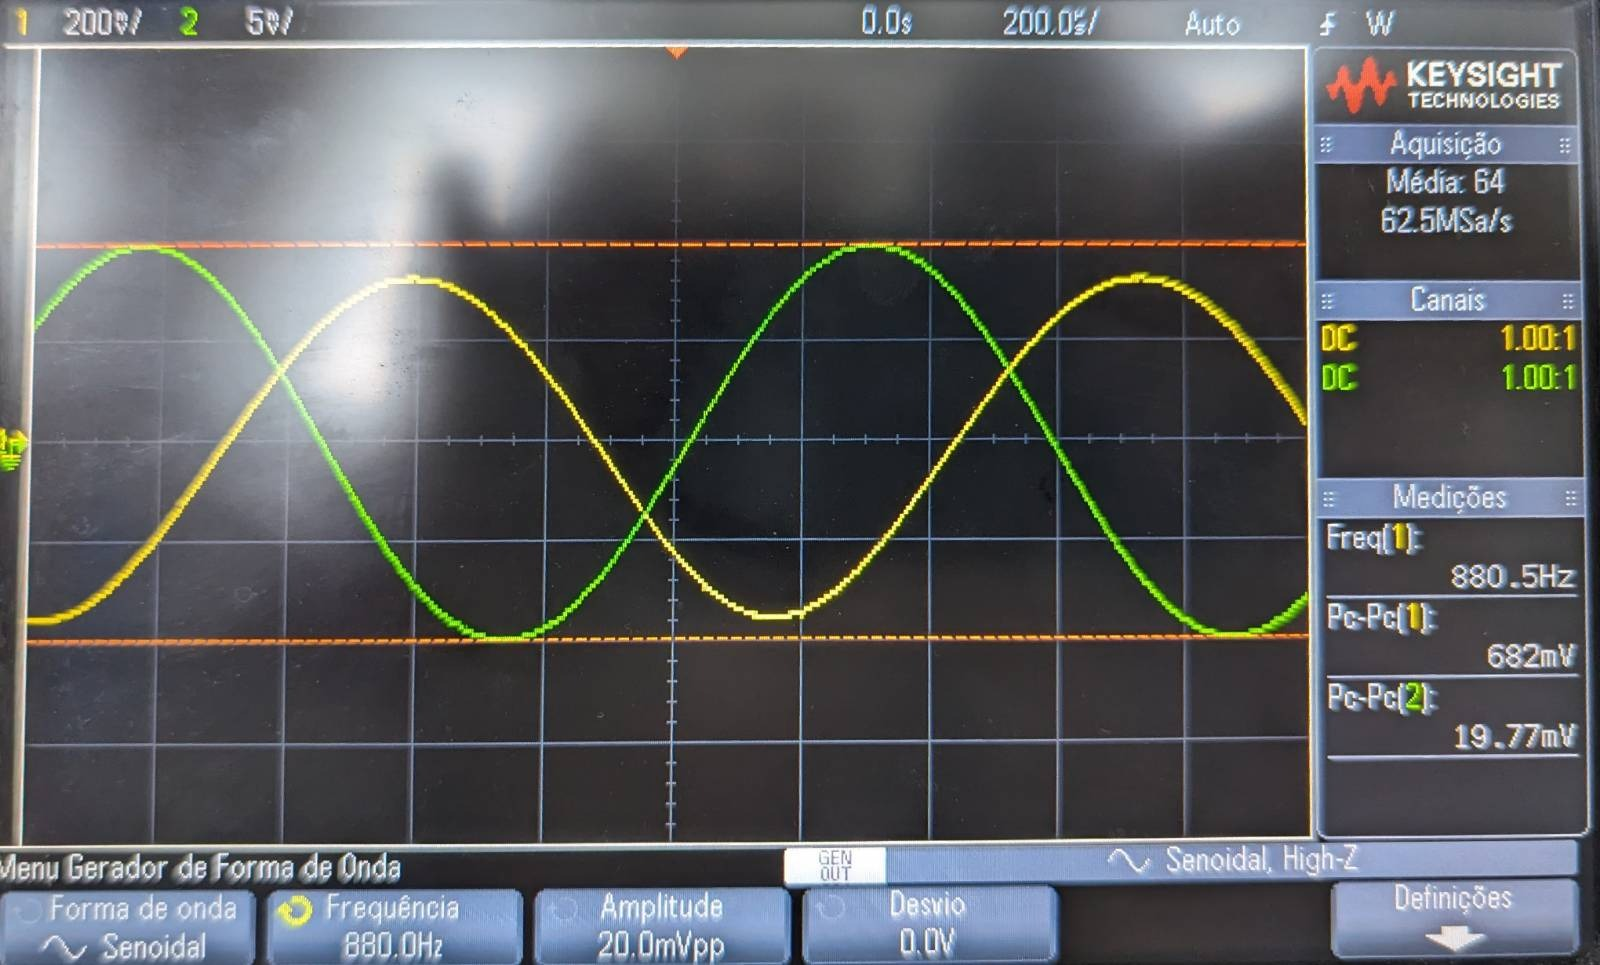
\includegraphics[width=0.5\columnwidth]{Images/frequencia_de_corte_baixa.jpeg}
    \caption{Circuito na frequência de corte.}
\end{figure}

\begin{figure}[H]
    \centering
    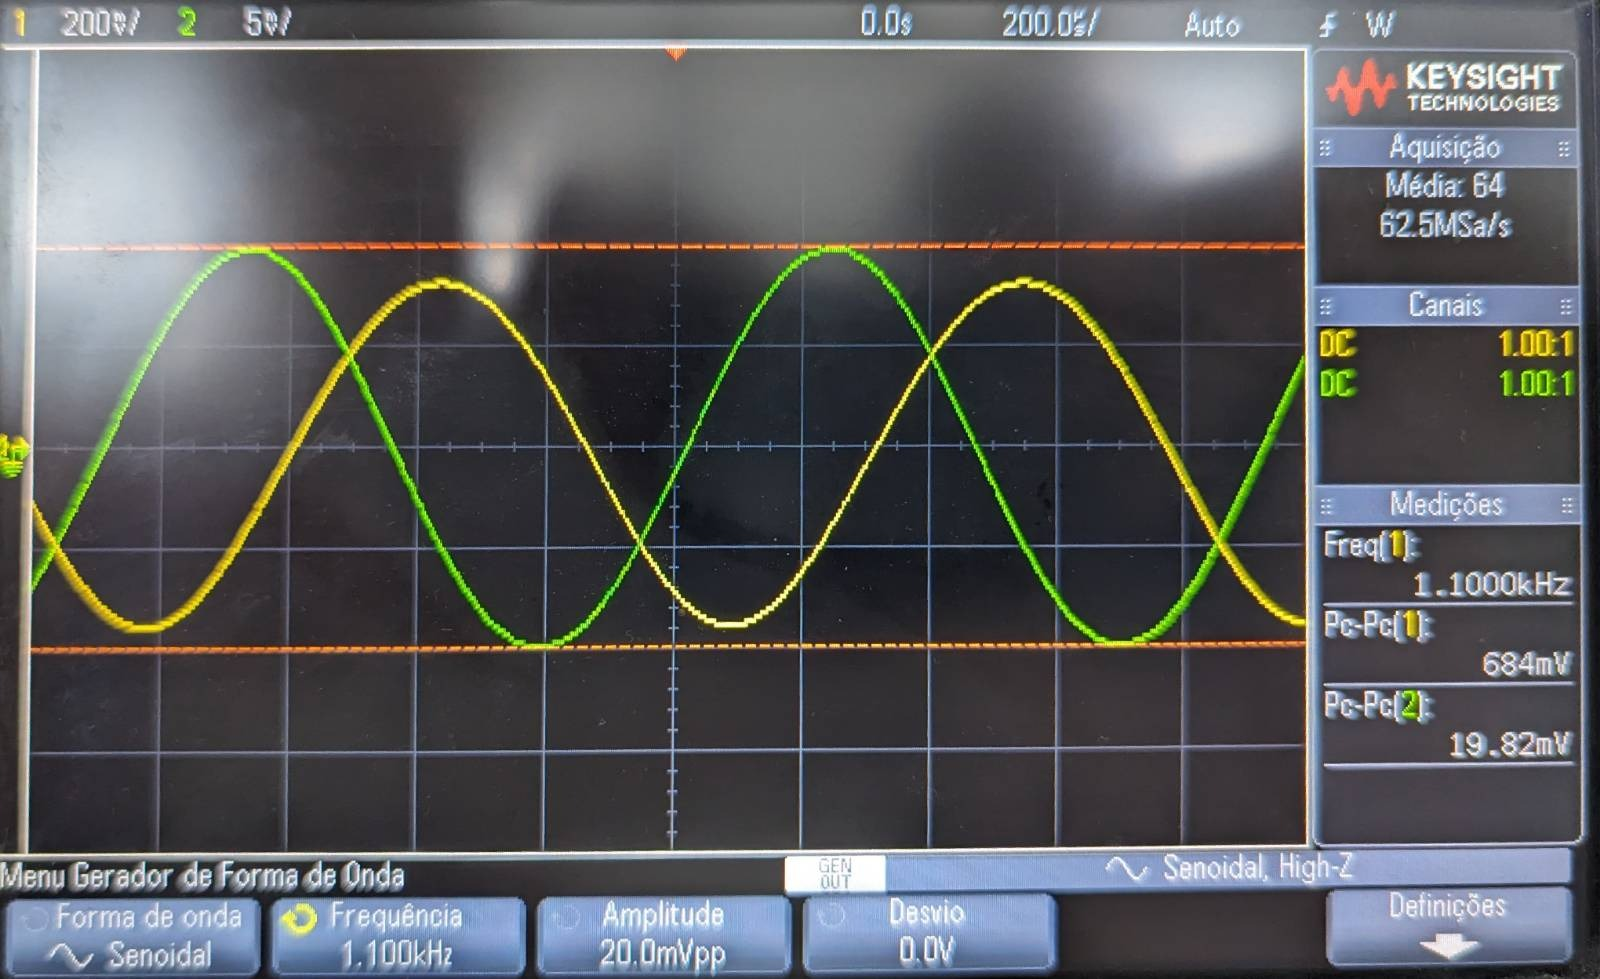
\includegraphics[width=0.5\columnwidth]{Images/freq_corte_C1_baixo.jpeg}
    \caption{Circuito na frequência de corte com $C_1$ 10 vezes menor.}
\end{figure}

\begin{figure}[H]
    \centering
    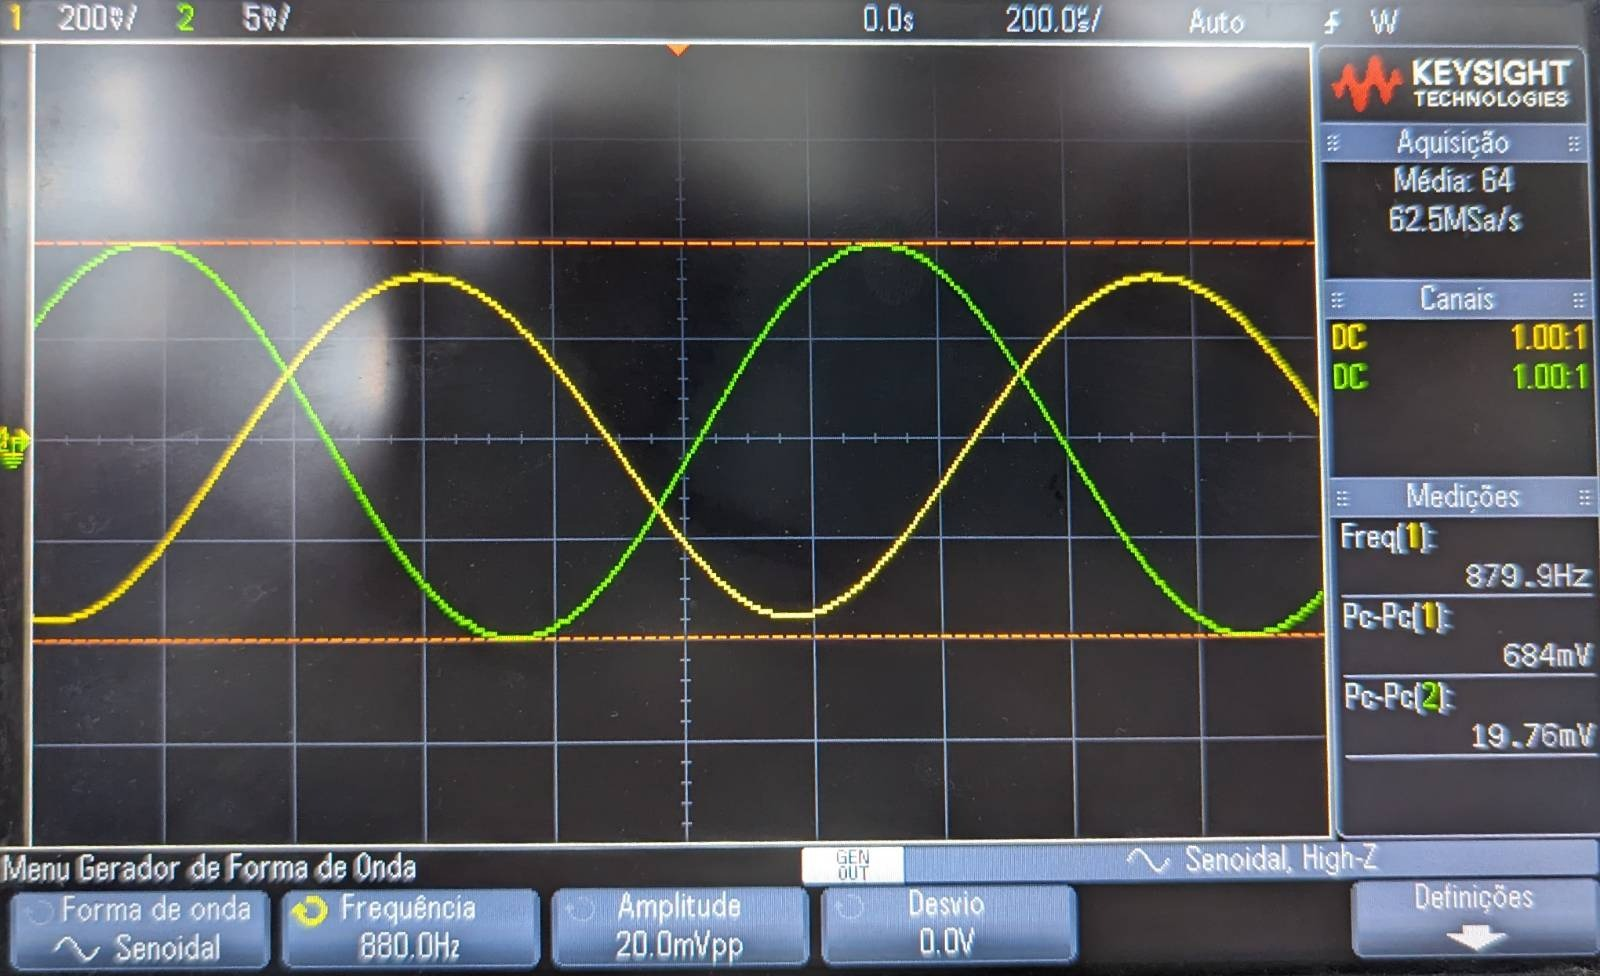
\includegraphics[width=0.5\columnwidth]{Images/freq_corte_C1_alto.jpeg}
    \caption{Circuito na frequência de corte com $C_1$ 10 vezes maior.}
\end{figure}


\begin{figure}[H]
    \centering
    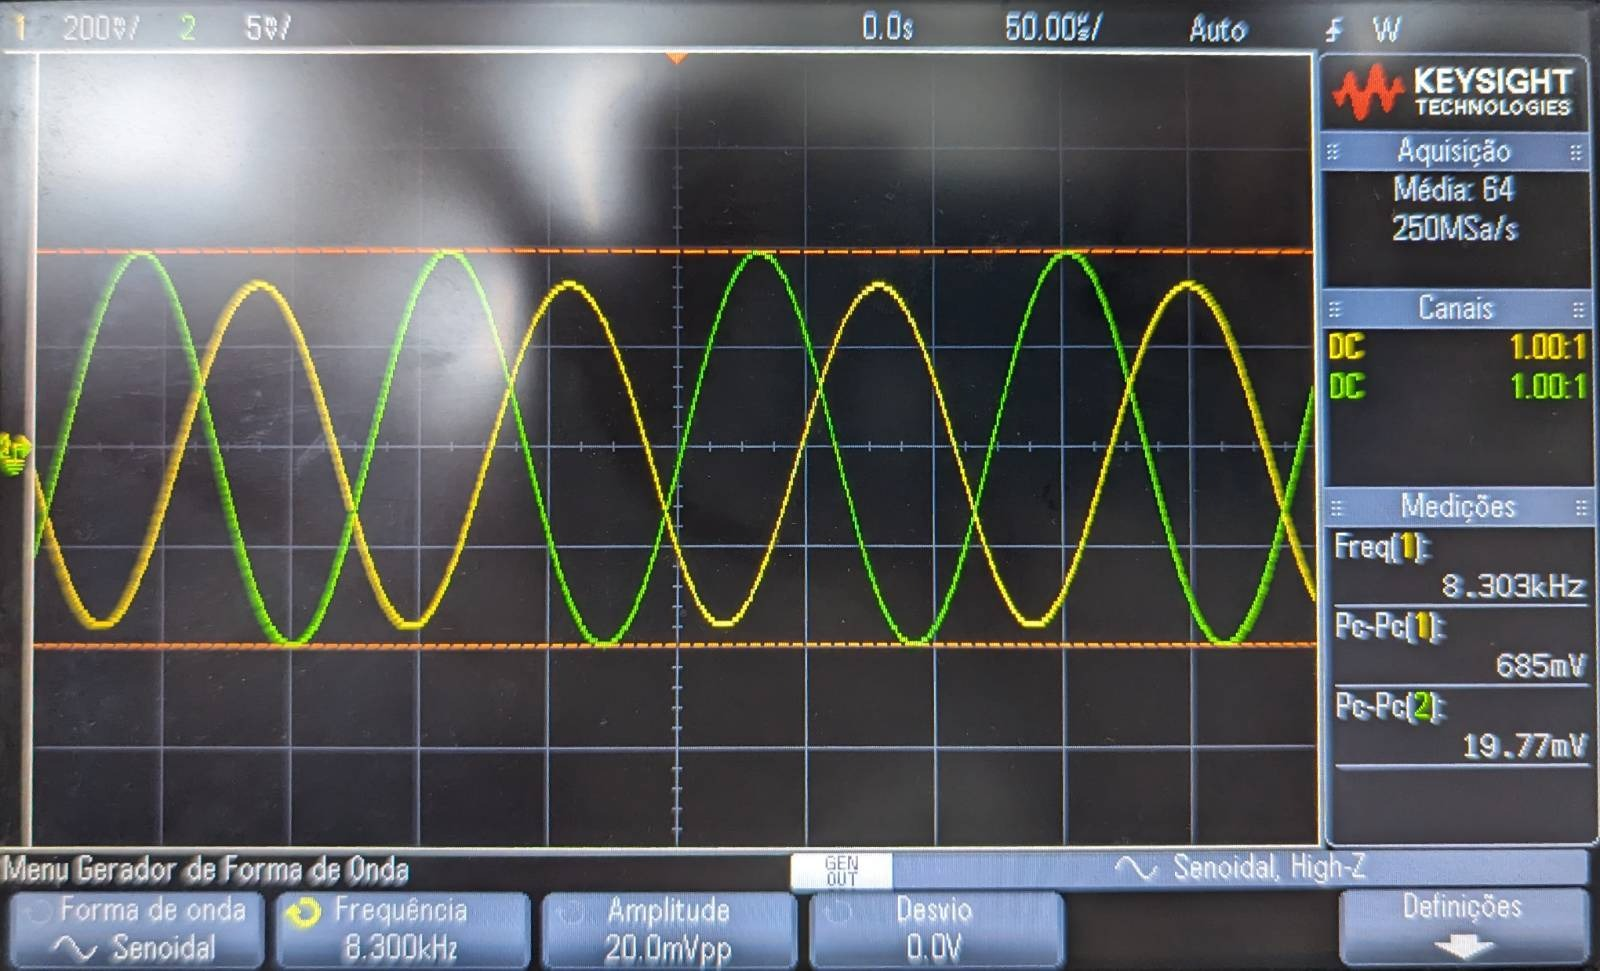
\includegraphics[width=0.5\columnwidth]{Images/freq_corte_C2_baixo.jpeg}
    \caption{Circuito na frequência de corte com $C_2$ 10 vezes menor.}
\end{figure}

\begin{figure}[H]
    \centering
    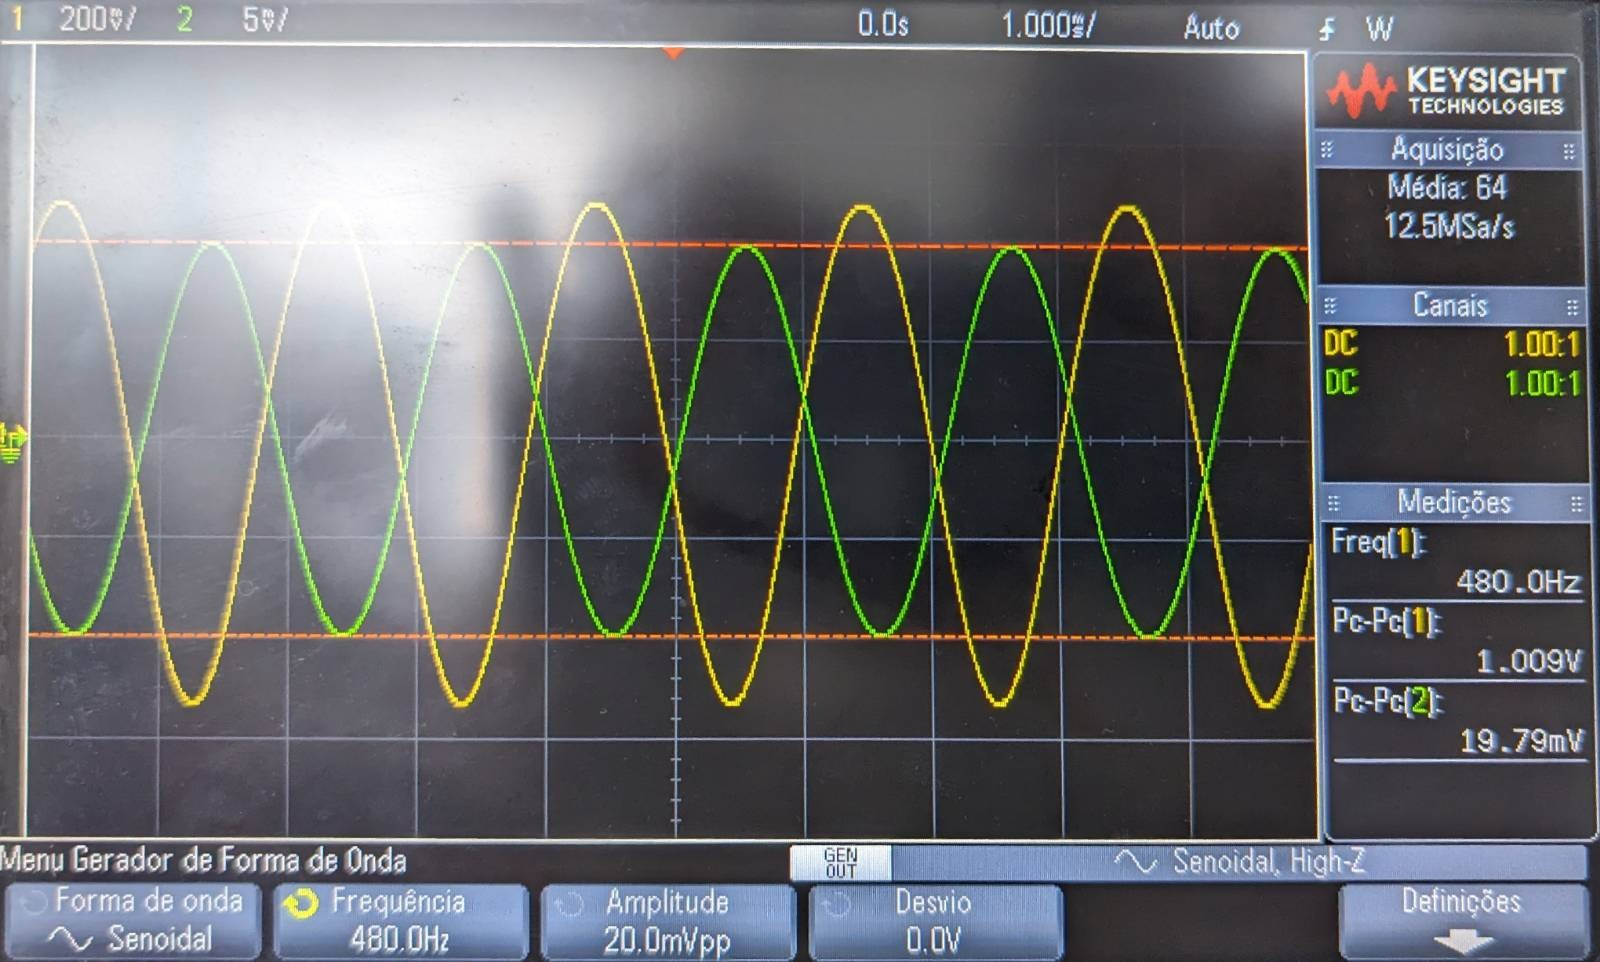
\includegraphics[width=0.5\columnwidth]{Images/freq_corte_C2_alto.jpeg}
    \caption{Circuito na frequência de corte com $C_2$ 10 vezes maior.}
\end{figure}


\begin{figure}[H]
    \centering
    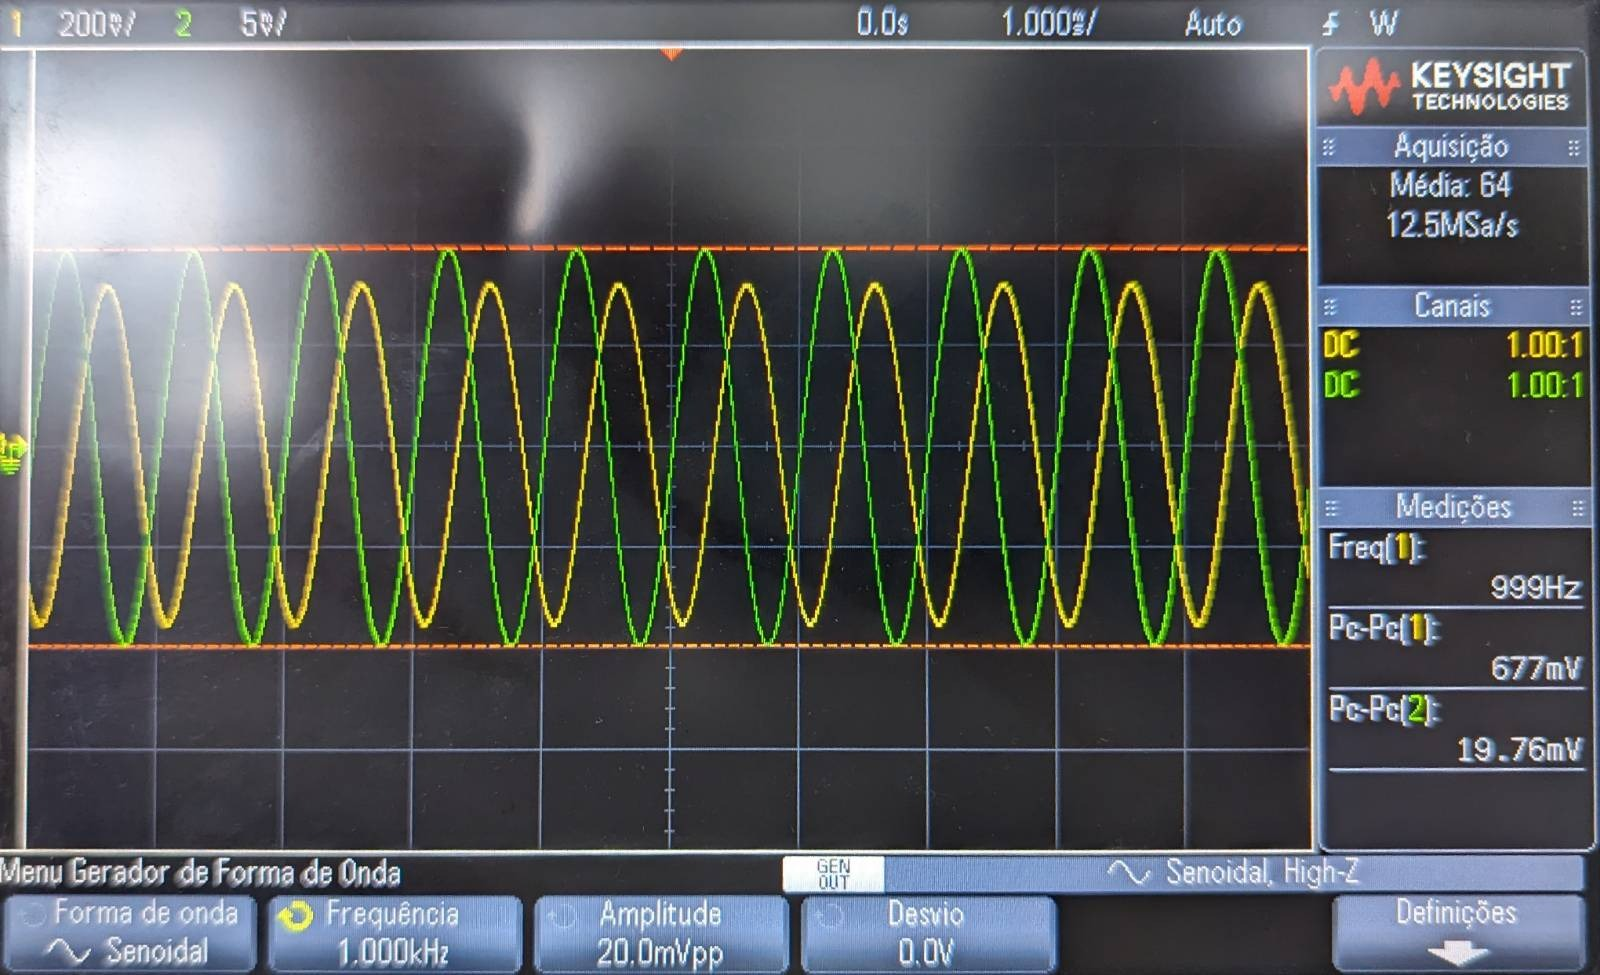
\includegraphics[width=0.5\columnwidth]{Images/freq_corte_C3_baixo.jpeg}
    \caption{Circuito na frequência de corte com $C_3$ 10 vezes menor.}
\end{figure}

\begin{figure}[H]
    \centering
    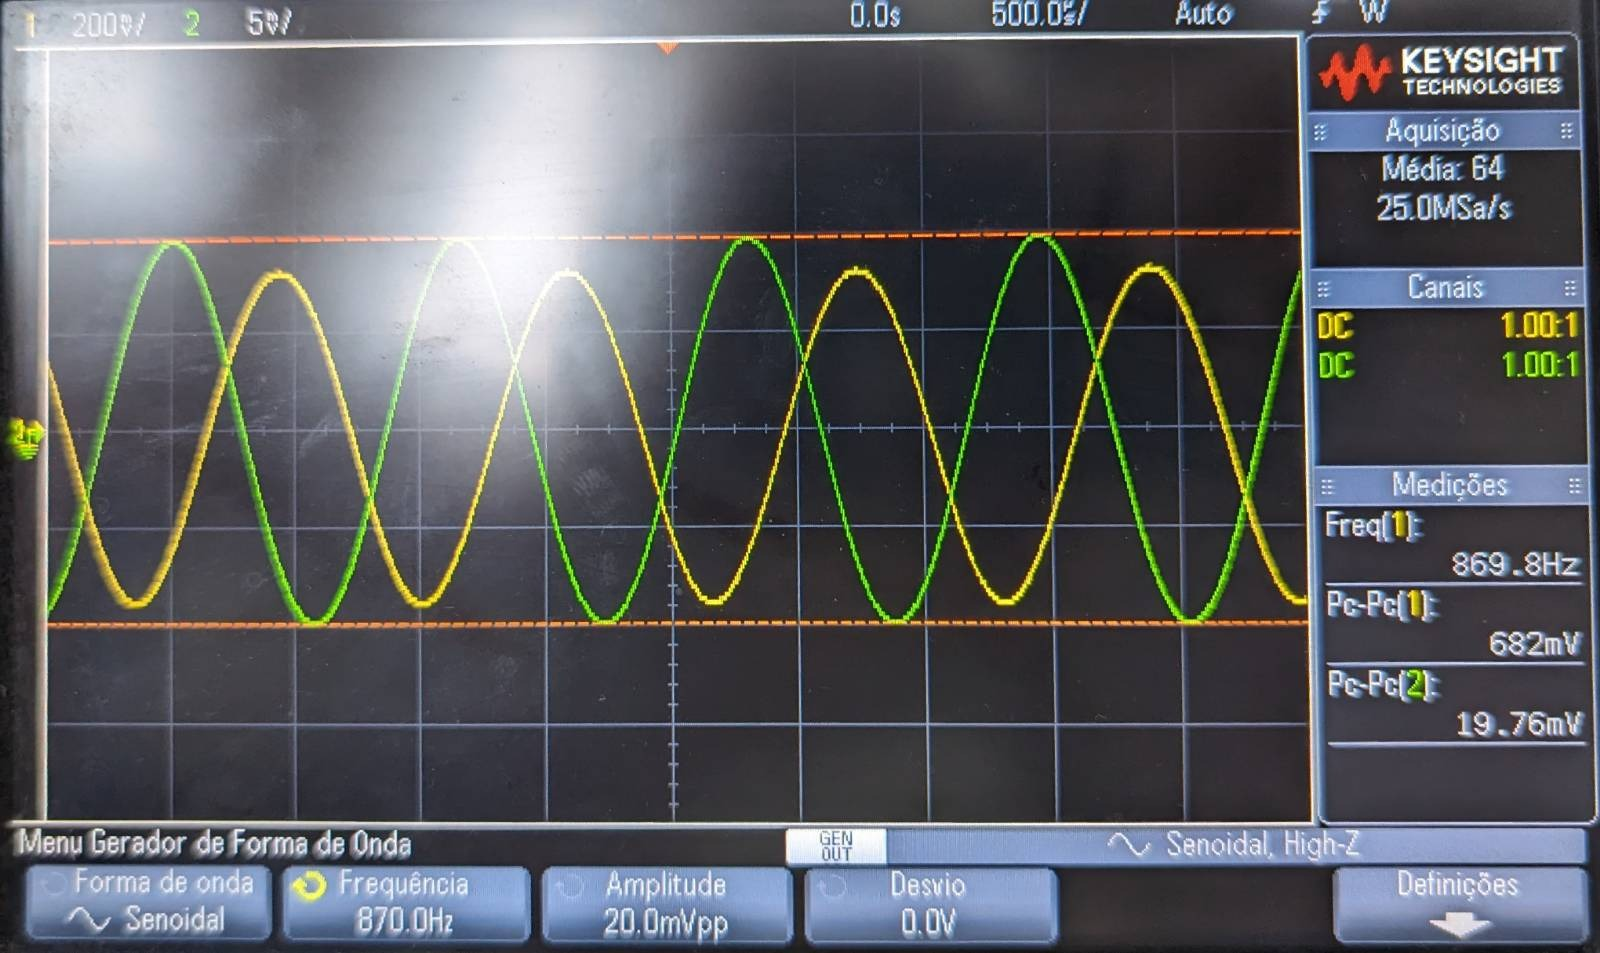
\includegraphics[width=0.5\columnwidth]{Images/freq_corte_C3_alto.jpeg}
    \caption{Circuito na frequência de corte com $C_3$ 10 vezes maior.}
\end{figure}